\chapter{Local Automatic Differentiation}
\label{ch:LocalAD}
This chapter will consider a different approach on how to use AD to solve PDEs. When solving PDEs using a finite volume method each cell will only depend on the neighbouring cells. In the \texttt{FAD} and \texttt{CJAD} implementations, the dependencies are stored in the discrete gradient and divergence operators. The implementations calculate the residual function value and corresponding Jacobian for the whole grid simultaneously by having a vector to store the values and sparse matrices for the Jacobians. Hence, when the discrete gradient and divergence operators are used in the calculation of the residual function in \autoref{ch:FlowSolver}, the Jacobian are obtained with the structure seen in \autoref{fig:flowSolverJacobian}. Local AD is an alternative approach that instead of calculating the residual function for all cells at once, using matrix and vector operations, it iterates through the grid and for each cell calculates the local residual. In the end it will perform exactly the same calculations as \texttt{FAD} and \texttt{CJAD}, but instead of having large vector and matrix calculations, we now have smaller calculations concerning only one cell, and its neighbours, at the time. This new approach is based on the same idea as how AD is implemented in OPM \emph{\citep{OPM}}, which, as said in introduction, is written in C and C++. The AD tool in OPM scales better when the simulations become larger and is the reason why it is used when creating efficient industrial simulators. It is hence interesting to see if you can write similar type of code in Julia and obtain better computational efficiency than what is achieved in MATLAB with MRST, as well as the methods I have already implemented in Julia. If this is possible, Julia could be a language where both prototyping and industrial simulators can be created, making the development process much more efficient. 

\section{Implementation}
\label{sec:LADImplementation}
To get a better understanding of how local AD works, it is best to look at how it is implemented\footnote{In the following I will explain a minor simplified implementation. This is to keep the focus on the essential parts of the implementation. The left out parts will be discussed in \autoref{sec:optimizingLocalAD}}. Like for \texttt{FAD} and \texttt{CJAD} I have implemented local AD using a struct called \texttt{LAD}:
\lstinputlisting{code/LAD_structSimple.jl}
Since we now only operate on one cell at the time, the implementation of local AD is simpler than for \texttt{FAD} and \texttt{CJAD}. The value of the AD-variable is now only a scalar and the Jacobian matrices are replaced by a vector of derivatives. These are the derivatives  with respect to the primary variables in the cell. For the single-phase flow solver in \autoref{ch:FlowSolver}, the derivatives vector will be of length one, as each cell only contains one primary variable (pressure). The implementation of \texttt{LAD} is, however, with \texttt{derivatives} as a vector. This is for the opportunity to implement more complex simulations like a two- or three-phase simulator, where each cell can contain multiple primary variables for the amount of water, oil and/or gas present in the cell (an example of a two-phase simulator can be seen in \autoref{sec:TwoPhaseSimulation}).

To make sure that each primary variable is initialized correctly, initialization of \texttt{LAD} variables is done with the \texttt{createVariable} function. This function creates a \texttt{LAD} variable with a value and a given number of derivatives. The derivative with respect to itself is set to $1.0$, whereas the other derivatives are zero.
\lstinputlisting{code/createVariable.jl}
The operators for the \texttt{LAD} struct are implemented similarly as explained in \autoref{ch:Implementation} for \texttt{FAD} and \texttt{CJAD}, but since we now, instead of having a Jacobian matrix, only have a vector of derivatives, the implementation is easier and follows the lines of the description from \autoref{sec:FADWithMultipleParameters}. 

\subsection{Flow Solver for Local AD}
\label{sec:FlowSolverLADImplementation}
Whereas the implementation of the local AD tool is easier than for \texttt{FAD} and \texttt{CJAD}, there is more work when calculating the residual functions. Since we no longer can use discrete gradient and divergence operators, but instead have to traverse through the grid cell by cell, we need a place to store the resulting residual values and the corresponding Jacobian. We also need a method to traverse through all the cells and calculate the contributions from each neighbouring cell.To create the flow solver from \autoref{ch:FlowSolver}, I have chosen to store the calculated values of the residual functions in another struct called \texttt{FlowSystem}:
\lstinputlisting{code/FlowSystem.jl}
This struct looks very similar to the other AD structs, except from \texttt{globalJac} being one single sparse matrix instead of a vector of sparse matrices. At this point you might not understand why it is quicker to calculate the residuals cell by cell compared to everything in one go. The key reason for this lies in the \texttt{FlowSystem} struct. Since we know that the structure of the global Jacobian will stay the same, we can reuse this sparse matrix structure throughout the whole simulation. Before the simulation begins, we use the grid variable \texttt{G}, which contains the information on which cells are neighbours, and build the correct structure of \texttt{globalJac} once and for all. When we later run the simulation, we only change the values inside of \texttt{globalJac}, but the structure stays the same. This reuse of \texttt{globalJac} will save a lot of memory allocations and hence consume less CPU time compared to \texttt{FAD} and \texttt{CJAD}, which both allocate new structs for each calculation. By creating a new constructor for \texttt{FlowSystem} that uses the grid variable \texttt{G}, the variables \texttt{eqVal} and \texttt{globalJac} will be allocated with the correct length and the correct structure before the simulation begins. For the grid in \autoref{ch:FlowSolver}, we have 1000 cells. This implies 1000 different pressure values and in addition we have the bottom-hole pressure (\texttt{bhp}) and the total production (\texttt{qS}). Hence, \texttt{eqVal} will be a vector of length 1002.

Now that \texttt{FlowSystem} stores the  values and Jacobian of the residual functions, we need a new function to traverse through all cells and perform the calculations. The function that will execute the calculations is \texttt{assembleFlowSystem!()}, where the exclamation mark is a Julia convention for a function that modifies its input parameters. The corresponding code can be seen below. I have removed all declarations of help variables and replaced the code for updating \texttt{FlowSystem} with comments to highlight the important parts of the function structure.
\lstset{numbers=left}
\lstinputlisting{code/assembleFlowSystem!.jl}
\lstset{numbers=none}
The input parameter \texttt{well} is a struct that contains all necessary information about the well. The first line in \texttt{assembleFlowSystem!()} resets \texttt{eqVal} and \texttt{GlobalJac} such that the structures are unchanged, but all the values are set to zero. Then, the function starts traversing through the grid and for every cell it adds up the contributions from all neighbouring cells. Be aware that the looping variable names \texttt{fromCell} and \texttt{toCell} can be a bit misleading when they represent bottom-hole-pressure and total production, as those primary variables do not belong to any cell. The intuitiveness of considering the flow from one cell to another is however considered more valuable than the issue that they will also represent bottom-hole-pressure and total production. The \texttt{eqVal} and \texttt{globalJac} variables are updated in line number 6, 8 and 10 inside the inner loop. As a reminder, the residual functions that \texttt{FlowSystem} eventually will represent are the functions \texttt{presEq}, \texttt{rateEq} and \texttt{ctrlEq} defined in \autoref{sec:setupGovEq}:
\lstinputlisting{code/governingEquationsPresSolver.jl}
In line number 6, \texttt{fromCell} and \texttt{toCell} are equal, but do not reference the bottom-hole-pressure or total production. Here, the first term in \texttt{presEq}, or the backward Euler term, is calculated. This is performed in an outer function called \texttt{timeDerivative()} that returns a \texttt{LAD} struct:
\lstinputlisting{code/timeDerivative.jl}
In \texttt{FAD} and \texttt{CJAD}, we made all the primary AD-variables before the simulation. We then used them as input parameters in the residual functions that returned new AD-variables which represented the values and Jacobians. With local AD, we create new primary AD-variables for the applicable cell inside the function we want to evaluate. For \texttt{timeDerivative()} we create a \texttt{LAD} primary variable that represents the pressure in the cell before we calculate the backward Euler term. When \texttt{timeDerivative()} has returned the new \texttt{LAD} variable, \texttt{assembleFlowSystem!()} adds the calculated value to the correct index in \texttt{eqVal} and the derivative value to the correct diagonal index in \texttt{globalJac}.

In line number 10, when \texttt{fromCell} and \texttt{toCell} are two neighbouring cells, the divergence term in \texttt{presEq} is calculated. Like for \texttt{timeDerivative()}, we create the primary AD-variables inside the function, but since we calculate the flux from one cell to another, we have to be careful with which direction we calculate the flux and which cell we want the derivative with respect to. Since the varying variables are named \texttt{fromCell} and \texttt{toCell}, it is natural that the function \texttt{flux()}, seen below, calculates the flux from \texttt{fromCell} to \texttt{toCell}. 
\lstinputlisting{code/fluxFunctionLocalAD.jl}
What needs to be chosen is which cell we want the derivative with respect to. The choice only affects which indices of the Jacobian the calculated derivatives should be added or subtracted to. In \texttt{flux()}, I have decided to calculate the derivative with respect to \texttt{fromCell}. The two first lines show the consequence of this, where \texttt{pFrom} is initialized with a derivative of $1$ and \texttt{pTo} as a constant. This choice leads to the following code for updating \texttt{FlowSystem} at line number 10 in \texttt{assembleFlowSystem!()}:
\lstinputlisting{code/fluxCodeLocalAD.jl}
The value of \texttt{fluxLAD} is added to \texttt{eqVal} and the derivative of the flux with respect to \texttt{fromCell} is added to \texttt{globalJac}. In addition we know that the flux from \texttt{fromCell} to \texttt{toCell} is the same as from \texttt{toCell} to \texttt{fromCell}, but with negative sign. This means that the derivative of the flux from \texttt{toCell} with respect to \texttt{fromCell} needs to be subtracted with \texttt{fluxLad.derivatives}. For a facet between two neighbours, we will with \texttt{assembleFlowSystem!()} calculate the value of the flux through the facet twice, only with different signs. You might think that we could save time by subtracting \texttt{fs.eqVal[toCell]} with \texttt{fluxLAD.val}, but since we also will need the opposite derivatives of this particular flux, there will small, or next to none, computational gain of exploiting this fact. In worst case it might actually become a slower implementation, as we would have had to keep track of which fluxes had been added to which cells. When the fluxes from all the neighbours have been added up for a cell, we have obtained the divergence in that cell. 

Line number 8 in \texttt{assembleFlowSystem!()} is the last line I have not commented and it is where the well equations, \texttt{rateEq} and \texttt{ctrlEq}, are handled. This line is executed if both \texttt{fromCell} and \texttt{toCell} either refer to one of the cells containing a well, the bottom-hole pressure, or the total production. The information on which cells fulfilling this condition lies in \texttt{well}. The calculation is performed by handling every case such that the correct residual functions, namely the \texttt{rateEq} or the \texttt{ctrlEq}, are calculated and added to the correct indices in \texttt{FlowSystem}.

Summed up, the calculation of the residual functions using local AD is based on two modules. The first is the actual AD tool with the \texttt{LAD} struct, and the second is \texttt{FlowSystem}, which keeps track of the global system and what calculations should be performed by the AD tool. With this approach, we loose some of the advantages using the other AD tools where the discrete residual functions looked very similar to the continuous case, like explained in \autoref{sec:setupGovEq}. The main structure of \texttt{assembleFlowSystem!()} will, however, be the same no matter what type of simulation, hence making modifications to the code, or building another simulator, will not demand a complete change of the code structure.

Now that the assemble of the governing equations are implemented, we need a main loop that performs the simulation. Since we have separated the assemble of the equations into a single function, the main loop will be very similar to the one outlined in \autoref{sec:setupGovEq}. The only difference is that instead of evaluating a residual function \texttt{F}, we assemble the equations using \texttt{assembleFlowSystem!()}. A pseudo code of the new main loop can be seen below. 
\lstinputlisting{code/FlowSimulatorLocalAD.jl}

\section{Optimizing Local AD}
\label{sec:optimizingLocalAD}
As explained in the beginning of this chapter, the main idea behind local AD is to reuse the Jacobian to save memory usage and extra memory allocations. The implementation given in \autoref{sec:LADImplementation} has nevertheless left out some small, but key parts of the implementation that will massively decrease the memory and CPU usage. This is purely implementation specific differences that have been left out to make the introduction to local AD more clear. It will not change the theory behind using local AD to solve PDE's.

\subsection{Dynamic VS Static Arrays}
The difference between a dynamic array and a static array is that a dynamic array can be extended or shortened as much as you like while a static array has a fixed length. Using a static array will give computational gain concerning speed and memory allocations compared to a dynamic array. This is because the compiler knows that a static array has the given fixed length forever and hence it can allocate the exact memory needed in advance and optimize the machine code accordingly. With a dynamic array, the compiler does not know if the array will grow larger, or smaller, and it is much harder to optimize the machine code. 

Julia has a package called \emph{\cite{StaticArrays}} that provides static arrays with the same abilities as the built-in arrays, but without the possibility for changing the size of the array. The package provides two types of vectors, \texttt{SVector} and \texttt{MVector}(for two-dimensional arrays it has the corresponding \texttt{SMatrix} and \texttt{MMatrix}). Both are static vectors, but \texttt{MVector} is mutable, meaning the values inside the vector can be changed, whereas the values inside an \texttt{SVector} are final once the vector is defined. This makes \texttt{SVector} ideal for \texttt{LAD.derivatives}, since when we perform operations on \texttt{LAD} variables, new \texttt{LAD} variables are returned.\footnote{For a multiphase simulation, a possible implementation can be each element in the global Jacobian being an \texttt{n}$\times$\texttt{n} matrix, where \texttt{n} is the number of primary variables in each cell. For this particular case, an \texttt{MMatrix} is optimal to use as we know the size of the matrices, but we want to change the values inside the matrix.} 

When the implementation is changed to use static vectors, it needs to know how long these vectors are. When building a simulator, it is not a problem to say in advance how many derivatives we need, and once the compiler knows this before compilation, it can optimize the machine code. OPM solves this by creating a template class containing the length of the gradient vector.\todo{Legg til både kilde og sjekk formulering} This ensures that the compiler always knows that for this simulator, the static vector will always have this fixed length. This is important because we do not want to create \texttt{LAD} structs with different lengths for \texttt{LAD.derivatives}. In addition, if we define this clearly, the compiler knows exactly how much memory is needed when we allocate a new \texttt{LAD} variable. By giving the compiler this information before compilation, we help the it to optimize the machine code. This will also make the implementation of the operators of \texttt{LAD} easier, as we know for certain that all \texttt{LAD} variables will have \texttt{derivatives} vectors with the same length. The best implementation I have found for this in Julia is to declare a global constant variable in the local AD module such that the new implementation of \texttt{LAD} becomes:
\lstinputlisting{code/LAD_struct.jl}
The disadvantage with this implementation is that the Local AD module needs to be modified to work for simulations with more primary variables for each cell. Since the implementations of the operators are unchanged, this modifications will only consist of changing the value of \texttt{NUM\_DERIV}. However, it would be better if Julia had the opportunity to pass in an argument into the \texttt{LAD} module. In this way the module could be compiled with any given value for \texttt{NUM\_DERIV}. As it is now, it is not possible to have one single \texttt{LAD} module and two different simulators with different number of primary variables, at the same time, in the same directory. A workaround could be to have multiple \texttt{LAD} modules with the only difference being the value of \texttt{NUM\_DERIV}. This would be a fully functional workaround, but not a very elegant one.

\section{Flow Solver Results for Local AD}
\label{sec:flowSolverWithLAD}
Now that \texttt{LAD} has been implemented with static vectors, it is interesting to see how the local AD method compares to \texttt{FAD} and \texttt{CJAD} in the simulation from \autoref{ch:FlowSolver}. Since the local AD technique from OPM, unlike the vectorized methods from MRST, is constructed with a main focus on computational efficiency, and since it is also assumed that Julia is supposed to run as fast as C, we expect that the local AD approach will give significant computational gain. This is unfortunately not the case with the implementation outlined in this chapter. Indeed, \texttt{LAD} performs worse than \texttt{CJAD} and similar to \texttt{FAD}. 

As explained in \autoref{sec:profiling}, profiling is an efficient way of finding the bottlenecks in a code, and this is a perfect example of when to use it - the code was expected to be faster, but it was not, so it is important to figure out if there is a small part of the code that is slow. \autoref{fig:profileSlowCreateVar} shows a screenshot of a profile result from running the flow solver simulation. The screenshot only contains blocks from the \texttt{flux()} function. Two blocks are marked with squares and two other blocks with brighter diagonal stripes. The blocks with squares are time spent in \texttt{createVariable()} and the brighter diagonal stripes are AD calculations in \texttt{flux()}.
\begin{figure}[H]
    \centering
    \begin{subfigure}[t]{0.75\textwidth}
        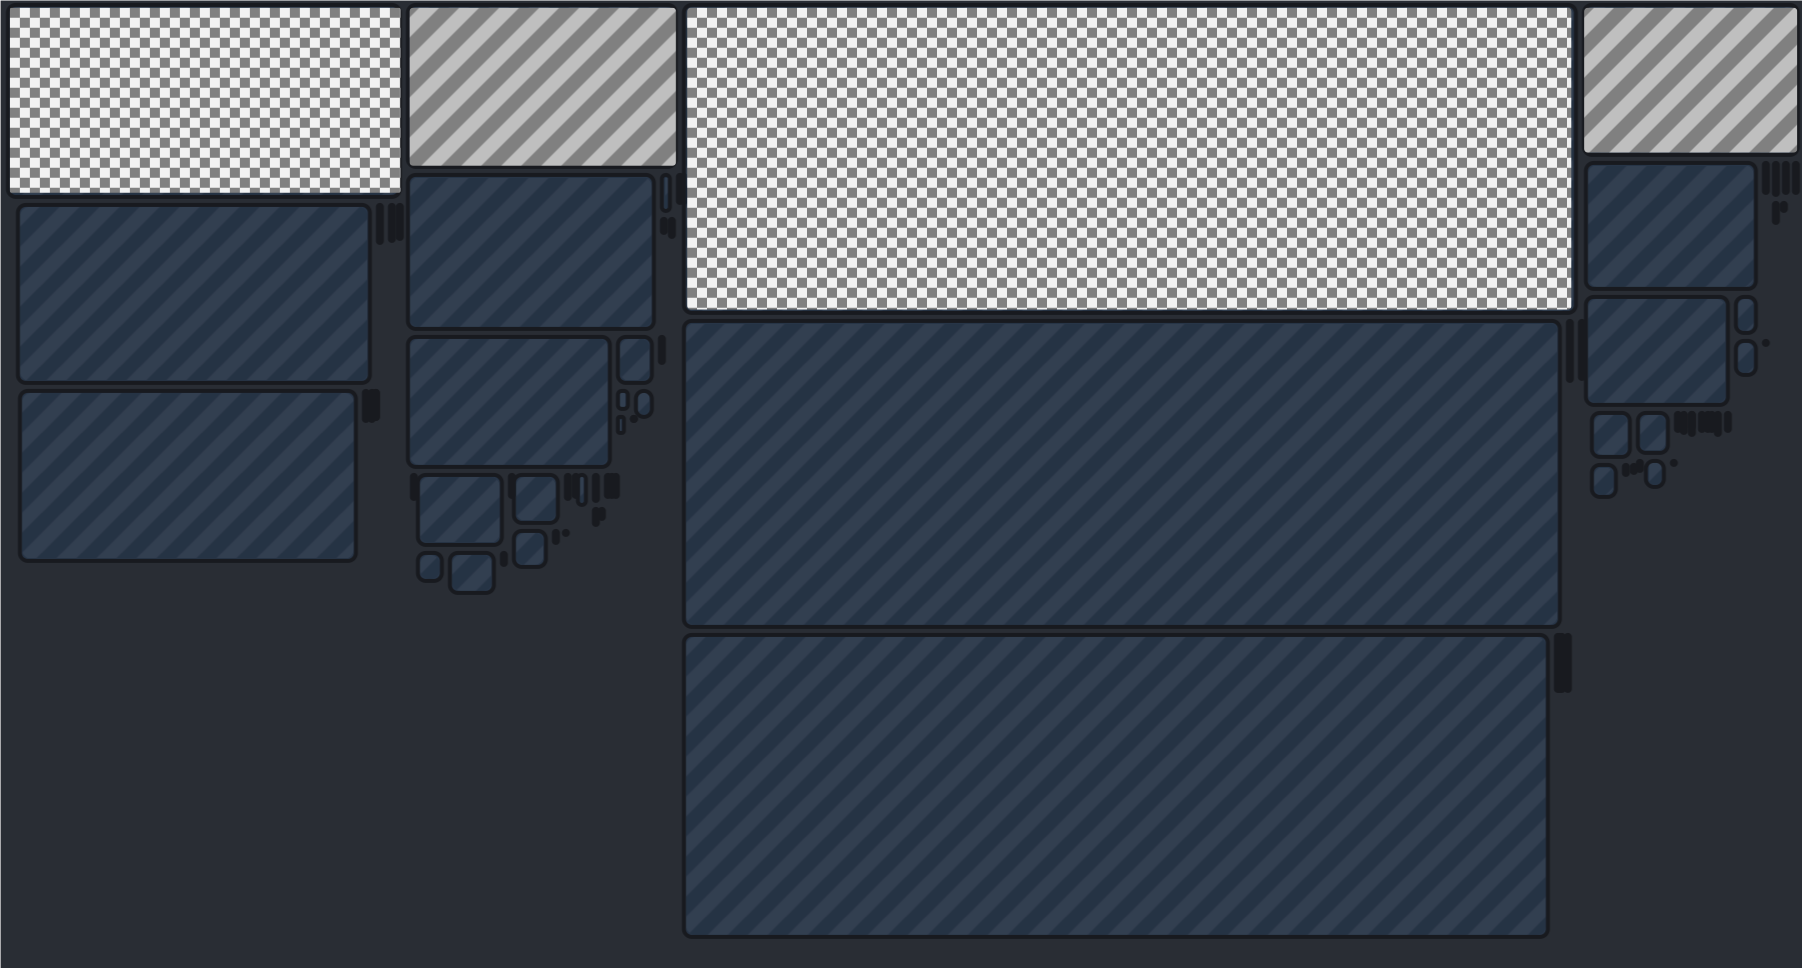
\includegraphics[height = 0.35\textheight, width=\textwidth ]{figures/profilingSlowCreateVariablesFlux.png}
        \caption{}
        \label{fig:profileSlowCreateVar}
    \end{subfigure}
    \hspace{0.06\textwidth}
    \begin{subfigure}[t]{0.18\textwidth}
        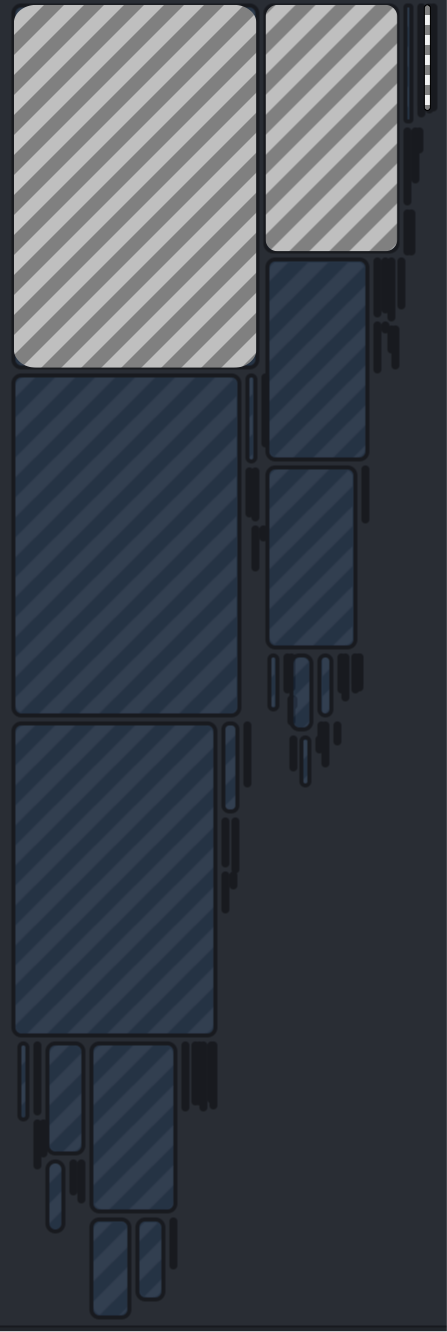
\includegraphics[height = 0.35\textheight, width=\textwidth]{figures/profilingFastCreateVariablesFlux.png}
        \caption{}
        \label{fig:profileFastCreateVar}
    \end{subfigure}
    \caption{The figures shows screenshots of the profile result from \texttt{flux()} in the flow solver simulation from \autoref{ch:FlowSolver}. The blocks marked with squares are time spent in \texttt{createVariable()} and the blocks with bright diagonal lines are calculations in \texttt{flux()}. \autoref{fig:profileSlowCreateVar} uses a slow version of \texttt{createVariable()} while \autoref{fig:profileFastCreateVar} uses a faster version.}
\end{figure}
It is suprising that creating a \texttt{LAD} struct should take more time than the actual AD calculations. This indicates that the \texttt{createVariable()} function is poorly implemented. If we look closer at the implementation, we see that we only want to create a static \texttt{Svector}, but we start by creating a dynamic vector of zeros, and then we modify the vector by changing one of the values to one. Finally, we convert the dynamic vector into a static \texttt{SVector} in the last line. The new implementation seen below is a Julia specific implementation, where the \texttt{SVector} is created immediately with correct values and without any use of dynamic vectors.
\lstinputlisting{code/createVariableFast.jl}
The new profiling result with the updated \texttt{createVariable()} can be seen in \autoref{fig:profileFastCreateVar}. The time spent in \texttt{createVariable()} is almost eliminated and we can see that approximately all the time spent in \texttt{flux} is used for AD calculations. This is what is expected as initialization should be far less time consuming than AD calculations. 

As discussed in \autoref{ch:FlowSolver}, by only looking at assembling of the residual functions, and not the full simulation, we eliminate the linear solver from the benchmark, and we get a better understanding of how efficient the AD tools are. \autoref{tab:FlowSolverAssemblyTestWithLAD} is the same table as \autoref{tab:FlowSolverAssemblyTest}, assembling the residual functions 100 times, but with the benchmarked time for Local AD added to the end of the table.
\begin{table}[htb]
    \centering
    \caption{Table with speed benchmarks of different AD methods assembling the "Single-Phase Compressible AD Solver" residual function 100 times for different discretizations.}
    \label{tab:FlowSolverAssemblyTestWithLAD}
    \def\arraystretch{1.5}
    \begin{tabular}{ccccc}
    \textbf{Number of cells} & \textbf{FAD} & \textbf{CJAD} & \textbf{MRST} & \textbf{Local AD}\\
        \hline
         $10\times10\times10$ & 0.9s & 0.4s & 0.6s & 0.07s \\  
         $20\times20\times20$ & 9.3s & 4.0s & 3.6s & 0.6s \\ 
         $30\times30\times30$ & 44.2s& 17.2s& 16.5s & 2.2s \\ \hline
    \end{tabular}
\end{table}
The table shows that the local AD approach is approximately six times faster than the other tested implementations, which is a significant improvement. This gives us an indication that Julia can be a language where we can quickly create new simulators using the high-level and user-friendly \texttt{CJAD} or a similar AD tool, and in the same language create more efficient simulators using a method like local AD. To confirm this, however, we need to test the performance for a larger problem than a single-phase pressure solver. In \autoref{sec:TwoPhaseSimulation}, I will test how local AD performs in Julia solving a two-phase problem with a more realistic grid structure. This will give a better indication on how well Julia is suited for creating high performance simulators.

\section{Two-Phase Incompressible Flow}
\label{sec:TwoPhaseSimulation}
Previously in this thesis, I have only looked at primary production, where we have single-phase flow, with oil as the only fluid present. As explained in the introduction, at most 30\% of the oil in the reservoir will be extracted unless we apply external forces to the reservoir. This normally consists of injecting either water, gas, or both, into the reservoir in a secondary production. There is also a third production phase called enhanced oil recovery or tertiary production, but as the purpose of this thesis is not oil recovery, but to see how the AD tools perform simulating oil recovery, I will not go into this subject. More detailed information about oil recovery can be found in \citet{lieMrstUrl}. I will also describe a simplified model of secondary production, where sufficient information for this example is that we want to simulate how water flows from an injector and into a reservoir full of oil. This will be simulated for a subregion of Model 2 from the 10th SPE Comparative Solution Project \emph{\citep{SPE10}}. This model represents a simplified reservoir geometry with somewhat exaggerated geological heterogeneity and was created as a challenging case to benchmark upscaling methods against each other.

The SPE10 (Model 2) grid is split into 85 layers. Each layer contains 60$\times$220 cells, making the total number of grid cells 1 122 000. To simplify the implementation, I will only look at a single layer, layer 5, making the problem two-dimensional with 13 200 cells. In differs from the grid in \autoref{ch:FlowSolver} in that the permeability and porosity varies throughout the grid. This will affect the path of the water flow. \autoref{fig:porositySPE10} shows the porosity in the grid and \autoref{fig:permeabilitySPE10} shows a logarithmic color plot of the permeability. Both figures also display the placement of the water injector in the center of the grid, and the four wells at each corner. \autoref{fig:porositySPE10} shows that the rock around wells P3 and P4 are very dense (low porosity) and \autoref{fig:permeabilitySPE10} naturally shows that the permeability is also low in this area. This gives us an expectation that the injected water will primarily flow to the left.
\begin{figure}[H]
    \centering
    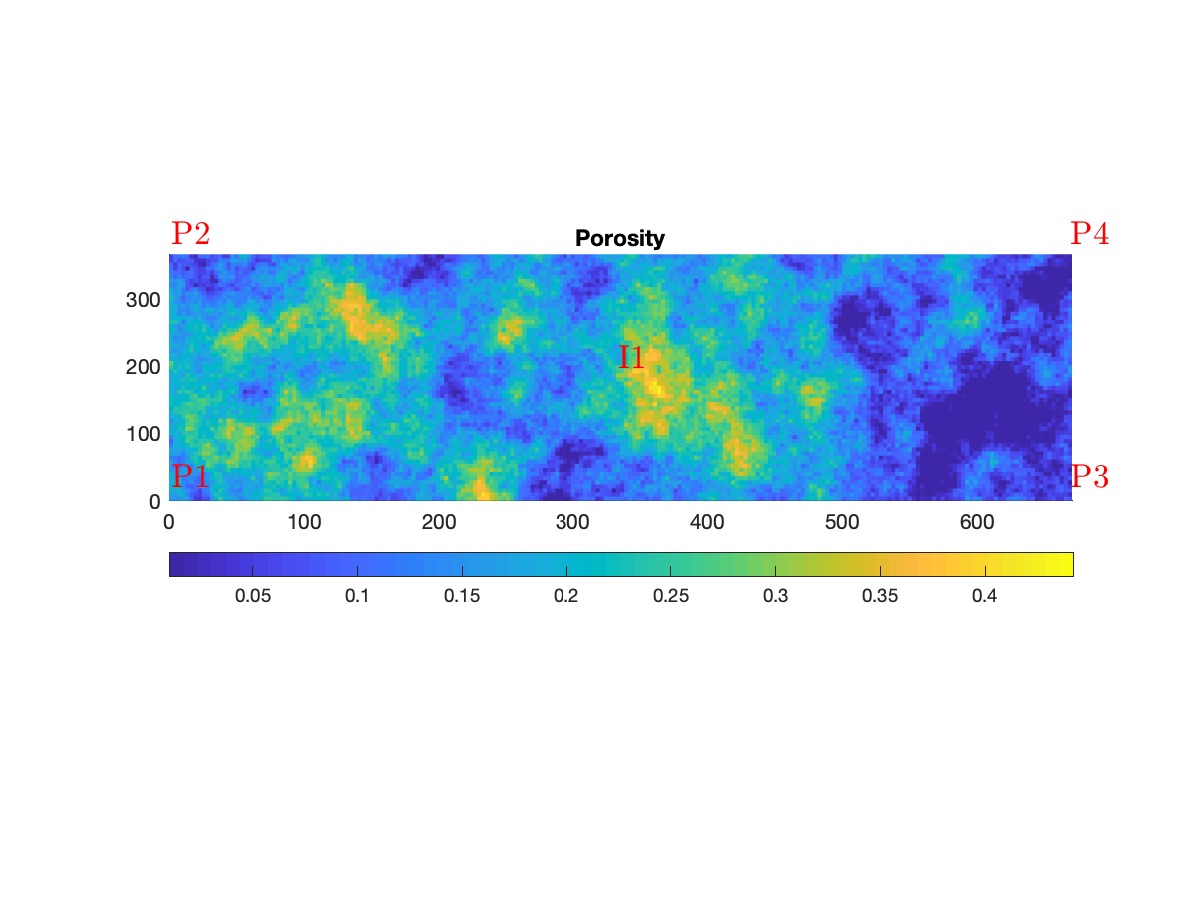
\includegraphics[width = \textwidth,clip=true,trim=20 130 10 90]{figures/porositySPE10.eps}
    \caption{Color plot of the porosity in the SPE10 grid.}
    \label{fig:porositySPE10}
\end{figure}
\begin{figure}[H]
    \centering
    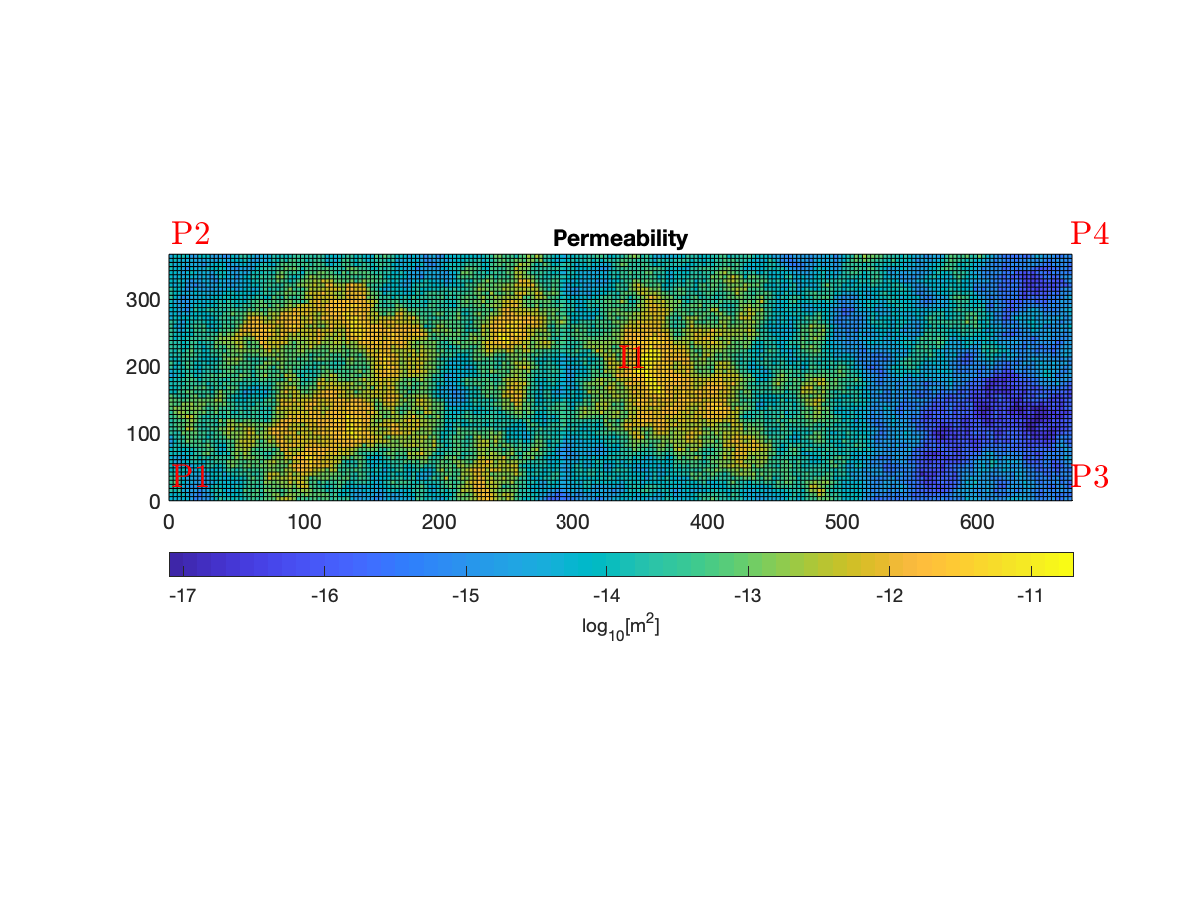
\includegraphics[width = \textwidth,clip=true,trim=20 120 10 90]{figures/permeabilitySPE10.eps}
    \caption{Logarithmic color plot of the permeability in the SPE10 grid.}
    \label{fig:permeabilitySPE10}
\end{figure}

\subsection{Derivation of the Governing Equations for Two-Phase Flow}
The governing equations for a two-phase flow are similar to the ones expressed in \autoref{ch:FlowSolver}, with some modifications. I will also make some simplifications to the model that I will note in the following derivation. Darcy's law, expressing the volumetric flow rate of a single-phase fluid, is given in \myeqref{eq:pressSolverDarcy}, but since our grid only has one layer, we neglect the gravity, and Darcy's law becomes
\begin{equation*}
    \textbf{v} = - \frac{K}{\mu}\nabla p.
    \label{eq:DarcyNoGravity}
\end{equation*}
However, now we need to separate between the flow of water, flow of oil and their overall flow. Before injection of water, each cell is only filled with oil. This implies that the amount of oil in a cell equals the pore volume in that cell. The pore volume is found by multiplying the total volume of the cell with the porosity, a number between zero and one. The volumetric fractions of water and oil, called the saturation, are defined similarly as the porosity as pointwise quantities, subject to the condition
\begin{equation*}
\sum_\alpha S_\alpha = 1
\end{equation*}
stating that the fluids fully occupy the available pore volume. In this two-phase situation, subscript $\alpha$ refers to the phase and can be either $o$ for oil or $w$ for water. As an example, in a cell without water, the oil saturation will be $S_o = 1$ and water saturation $S_w = 0$.  The effective permeability a fluid phase experiences when flowing through a medium partially occupied by another mobile fluid phase can be significantly lower than if the phase flows alone. The reduction is generally not linear in $S$ and hence we cannot find the phase flux by simply multiplying Darcy's law with the saturation. To get an expression for the phase flux, we introduce the property relative permeability. Relative permeability is often represented as a tabulated quantity, but herein I have chosen to use one of the simplest commonly used analytic models, given by
\begin{equation*}
k_{r\alpha} = S_\alpha^2,
\end{equation*}
for both water and oil. The flux for phase $\alpha$ is then given by the modified Darcy's law
\begin{equation*}
\textbf{v}_\alpha = - \frac{Kk_{r\alpha}}{\mu_\alpha}\nabla p_\alpha = -K\lambda_\alpha\nabla p_\alpha.
\end{equation*}
Here, $p_\alpha$ is the pressure for the given phase and $\lambda_\alpha$ is called the mobility of phase $\alpha$. The difference between oil and water pressure is given by the capillary pressure, $p_c = p_o - p_w$. For an oil--water system, the capillary pressure would cause water to rise in the reservoir. However, in this model we neglect capillary pressure so that the oil- and water pressures are considered to be equal. Now that we have an expression for the phase flux, we obtain the conservation equation for each phase:
\begin{equation}
    \frac{\partial}{\partial t}(\phi \rho_\alpha S_\alpha) + \nabla\cdot(\rho_\alpha\textbf{v}_\alpha) = \rho_\alpha q_\alpha.
    \label{eq:continuityEqMultiPhase}
\end{equation}
If you remove $\alpha$ from \myeqref{eq:continuityEqMultiPhase}, it becomes the same equation as \myeqref{eq:continuityEqPressure}, except that in \myeqref{eq:continuityEqPressure}, $\rho$ is inside of the source term $q$. In our two-phase example we assume both phases to be incompressible such that the governing equations are given by
\begin{equation}
    \frac{\partial}{\partial t}(\phi S_\alpha) + \nabla\cdot\textbf{v}_\alpha =  q_\alpha, \hspace{1em} \alpha \in o, w.
    \label{eq:continuityEqsMultiPhaseIncomp}
\end{equation}
Since $S_o = 1 - S_w$, the equations from \myeqref{eq:continuityEqsMultiPhaseIncomp} contain only two unknown variables, the saturation, for either water or oil, and the pressure. This means that we have enough equations to solve for the unknown variables and we could solve them simultaneously. However, the equations are strongly coupled, and for this example we will rather reformulate the two equations as an elliptic equation describing the pressure and a hyperbolic equation describing the water saturation, since these reformulated equations are less coupled. This gives us the opportunity to solve the equations separately using an operator splitting method I will explain later. We start by obtaining an equation for the pressure. By adding the two equations from \myeqref{eq:continuityEqsMultiPhaseIncomp} we obtain
\begin{equation*}
    \phi \frac{\partial}{\partial t}(S_o + S_w) + \nabla\cdot(\textbf{v}_o + \textbf{v}_w) = q_o + q_w.
\end{equation*}
Since $S_o + S_w = 1$, we can remove the time dependent term, and by defining the total flux as
\begin{equation*}
    \textbf{v} = \textbf{v}_o + \textbf{v}_w = -K\lambda_o\nabla p -K\lambda_w\nabla p = -K\lambda\nabla p,
\end{equation*}
and the total source term as $q = q_o + q_w$, we obtain the pressure equation:
\begin{equation}
    -\nabla\cdot(K\lambda\nabla p) = q.
    \label{eq:pressureEq}
\end{equation}
Next, we derive the equation for the water saturation. \myeqref{eq:continuityEqsMultiPhaseIncomp} with $\alpha = w$ gives one formulation, but we want an expression that depends on the total flux, and not the water flux. The reason for this will be explained later. To find a relation between the water flux and the total flux, observe that the difference between the water flux, multiplied with the mobility of oil, and the oil flux, multiplied with the mobility of water, is equal to zero.
\begin{align*}
    \lambda_o\textbf{v}_w - \lambda_w \textbf{v}_o = \lambda\textbf{v}_w - \lambda_w\textbf{v} &= (\lambda_o + \lambda_w)\textbf{v}_w - \lambda_w(\textbf{v}_o + \textbf{v}_w) \\
    &= \left(\lambda_o\lambda_w + \lambda_w^2 - (\lambda_w^2 + \lambda_w\lambda_o)\right)\left(-K\nabla p\right) = 0.
\end{align*}
This gives us the relation 
\begin{equation*}
    \textbf{v}_w = \frac{\lambda_w}{\lambda_o + \lambda_w}\textbf{v} = f_w\textbf{v},
\end{equation*}
where $f_w$ is called the fractional water flow. Inserting the expression for water flux into the conservation law for the water phase, given in  \myeqref{eq:continuityEqsMultiPhaseIncomp}, we obtain the transport equation:
\begin{equation}
    \phi \frac{\partial S_w}{\partial t} + \nabla\cdot\left(f_w\textbf{v}\right) =  q_w.
    \label{eq:transportEq}
\end{equation}
Even though we now have separated the governing equations into a pressure equation and a transport equation, they are still coupled. \myeqref{eq:pressureEq} is depending on the water saturation in the total mobility $\lambda$ and \myeqref{eq:transportEq} is depending on the pressure in Darcy's law for the flux, \textbf{v}. However, this coupling is weaker than in \myeqref{eq:continuityEqsMultiPhaseIncomp}, and this weaker coupling opens up the opportunity to use an operator splitting method. This consist of first solving the pressure equation, holding the saturation constant. Then, when we have found the correct pressure, we hold the pressure and the total flux constant for a (short) time step and solve the transport equation. Since the total flux is held constant as well when solving the transport equation, the total flux calculated in the pressure equation can be used to solve the transport equation. This is why we wanted to find an expression for the water flux, given by the total flux. When the water saturation is updated, we continue with the next time step by solving the pressure equation for constant saturation, and so on.

\subsection{Implementation of a Two-Phase Solver}
In the implementation of the two-phase simulator for the SPE10 grid, a lot will be very similar as for the previous single-phase implementation from \autoref{sec:FlowSolverLADImplementation}. The \texttt{FlowSystem} struct is replaced with a \texttt{TwoPhaseSystem} struct that hold the residuals and Jacobians for both equations. In addition to this, for implementation convenience purposes, it also holds the current pressure and water saturation:
\lstinputlisting{code/TwoPhasSystem.jl}
Naturally, instead of having a single function to assemble equations, the simulator now has two, called \texttt{assemblePressureEquations!()} and \texttt{assembleTransportEquations!()}. These are implemented with the same structure as \texttt{assembleFlowSystem!()}, only that the equations calculated are different. The main loop that controls the simulation is also extended. As explained above, the pressure equation and the transport equation are solved interchangeably and the implementation of this can be seen below.
\lstinputlisting{code/TwoPhaseSimulator.jl}

\subsection{Two-Phase Solver Results}
Even though we are most interested to see how the AD tools perform, we also have to see what we are simulating to make sure that it is correct implemented. \autoref{fig:waterSatResultsSPE10} shows the development of the water saturation in the SPE10 grid, for a simulation over three years. The total amount of water we have injected after three years is 0.135 of the total pore volume in the reservoir. As we can see from the figure, the assumption we had that the water will flow to the left was correct. We can also see that it follows paths in the reservoir that are optimal for the water to flow. One example that is easy to spot, is that the water, at least in the beginning, avoids the area straight left of the injector. If we go back to \autoref{fig:porositySPE10} and \autoref{fig:permeabilitySPE10}, we can see that in this area, both the porosity and the permeability are low.
\begin{figure}
    \centering
    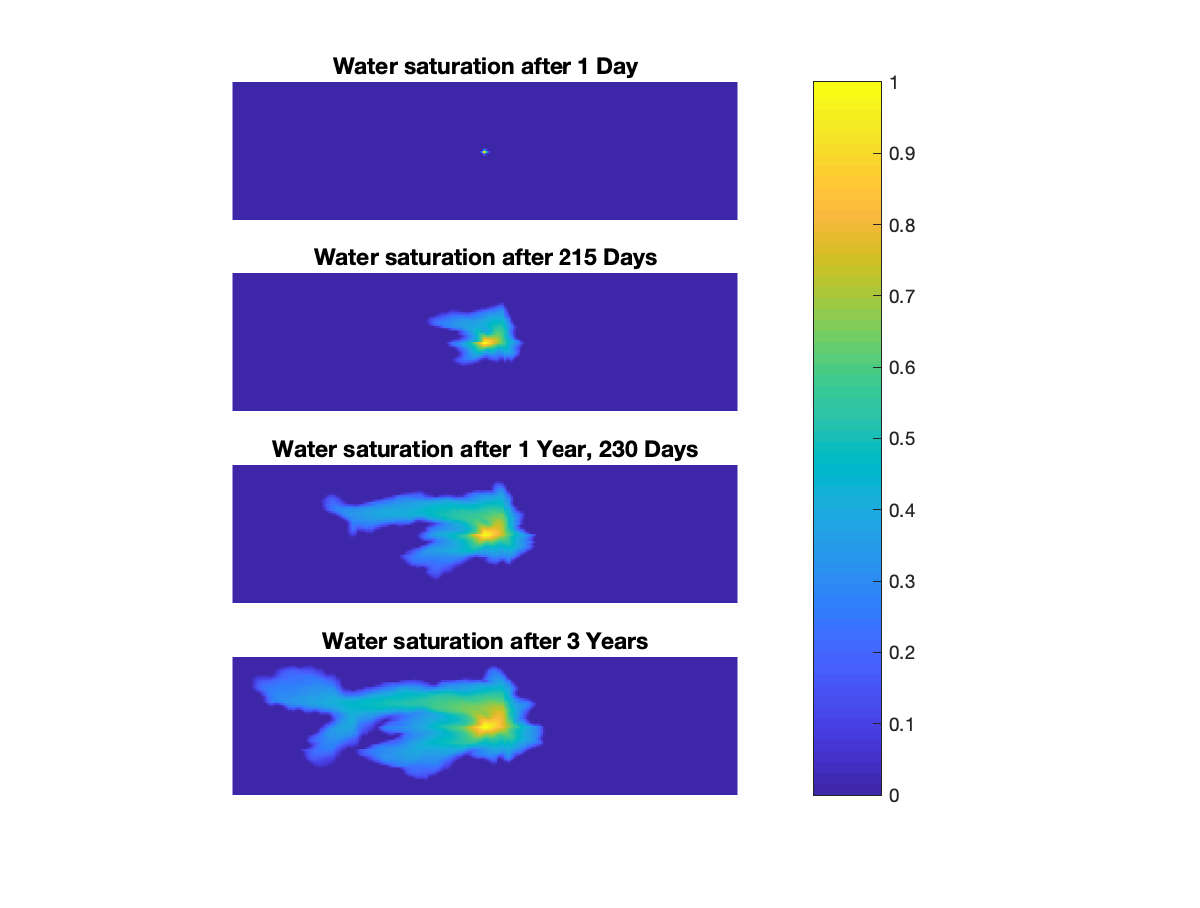
\includegraphics[width = .8\textwidth,clip=true, trim=100 30 100 10]{figures/waterSaturation4x1ThreeYears.eps}
    \caption{Color plot of the water saturation development in the SPE10 grid over a period of three years. Total injected water after three years is 13.5\% of the total pore volume in the reservoir.}
    \label{fig:waterSatResultsSPE10}
\end{figure}
\todo[inline]{Gjøre plottene større og med mindre svarte kanter. Gjøres enkelt ved å sette 'edgeColor','none' som ekstra argument til plotCellData}
To benchmark the AD performance in the two-phase simulation, I have, similar to the previous benchmarks, separated the AD calculations from the linear solver. The simulation in \autoref{fig:waterSatResultsSPE10} used approximately 150 time steps, and for each time step, the Newton--Raphson method used two iterations to solve the pressure equations and approximately six iterations to solve the transport equations. The benchmark I have performed is essentially this same simulation, but without the linear solver and the update of the pressure and the water saturation. This will give us a good estimation on how much time the simulator spend on AD during the simulation. Since the benchmark does not update the pressure and water saturation, it could have been the case that the compiler figure out that there is no need to perform all calculations, and that it for example is enough doing it only once. However, this is tested and it is not the case. The benchmark is performed for the local AD method, the \texttt{CJAD} method and for the AD tool in MRST. The results of the benchmark can be seen in \autoref{tab:TwoPhaseBenchmark}. The table shows that \texttt{CJAD} and MRST perform similar, with approximately 30 seconds in total. The local AD outperforms both the two other methods, and for this benchmark, it is approximately five times as fast.
\begin{table}[htb]
    \centering
    \caption{Write caption}
    \label{tab:TwoPhaseBenchmark}
    \def\arraystretch{1.5}
    \begin{tabular}{ccc}
    \textbf{Local AD} & \textbf{CJAD} & \textbf{MRST}\\
        \hline
        5.89s & 31.97s & 30.15s \\  
        \hline
    \end{tabular}
\end{table}
This result gives us an even stronger indication that Julia is a language that can be used both to create quick simulators using a high-level and user-friendly AD methods, like what is implemented in MRST, as well as to create more performance strong simulators, using low-level implementations like in OPM.

\todo[inline]{Se på parallellisering for lokal AD?}